\section{Результаты численного моделирования}

В настоящем разделе описаны результаты двух видов расчетов. Во-первых, проведенной верификации модели экипажа на плоскости с регуляризованным сухим трением в сравнении с безынерционной моделью (см. Приложение к главе 1, а также~\cite{ZobovaTatarinovPMM,Borisov2011}). Сравнение проведено при стремлении доли массы ролика в общей массе омни-колеса к нулю. Во-вторых, качественного сравнения движения экипажа на плоскости с вязким трением с достаточно большим коэффициентом и движения модели, построенной в главах 1 и 2.

\subsection{Верификация модели с сухим трением}

Для проверки взаимной корректности безынерционной модели и модели с сухим трением проведены численные испытания, в которых, при прочих равных, изменялась величина $\massrel$ -- отношение массы одного ролика к массе колеса в целом. В этом случае оказалось, что при уменьшении данного параметра движение экипажа и омни-колес приближаются к соответствующим решениям задачи Коши, получаемым в силу дифференциальных уравнений движения, используемых в работе~\cite{Borisov2011}, в которых динамика роликов не учитывается. При этом остальные параметры экипажа, такие как массы его частей, их моменты инерции, геометрические размеры, положения, а также начальные данные -- скорость центра масс и угловая скорость платформы, задавались согласованными между двумя моделями. Как и в главах 1 и 2, рассматривается симметричная конфигурация экипажа. Однако концы роликов в данном рассмотрении не усекаются: в силу выбора модели контактных сил и построенного явного алгоритма отслеживания контакта, особенность на острии ролика не препятствует проведению расчетов. Количество роликов $n$ равно $4$. Рассмотрены два типа начальных условий $\vec{v}(0) = (v_0, 0, 0)^T, \omega(0) = \omega_0$ (см. рис.~\ref{fig:nu_fric}):
\begin{enumerate}
\item центр платформы экипажа имеет начальную поступательную скорость в направлении одного из колес, и угловая скорость платформы равна нулю (ожидаемый результат - центр масс экипажа движется вдоль оси $Ox$, экипаж не вращается),
\item платформа экипажа имеет ненулевую угловую скорость вокруг вертикальной оси, проходящей через центр масс экипажа, скорость центра масс равна нулю (ожидаемый результат - экипаж вращается вокруг своей вертикальной оси симметрии, и центр масс покоится).
\end{enumerate}
За единицу безразмерной массы принята масса диска колеса. Безразмерная масса платформы при этом равна $3.3$. Отношение $\massrel$ массы ролика к общей массе колеса в обоих случаях принимало значения от $10^{-6}$ до $10^{-1}$ с шагом $1$ по показателю степени.

% \begin{figure}[!ht]
%     \centering
%     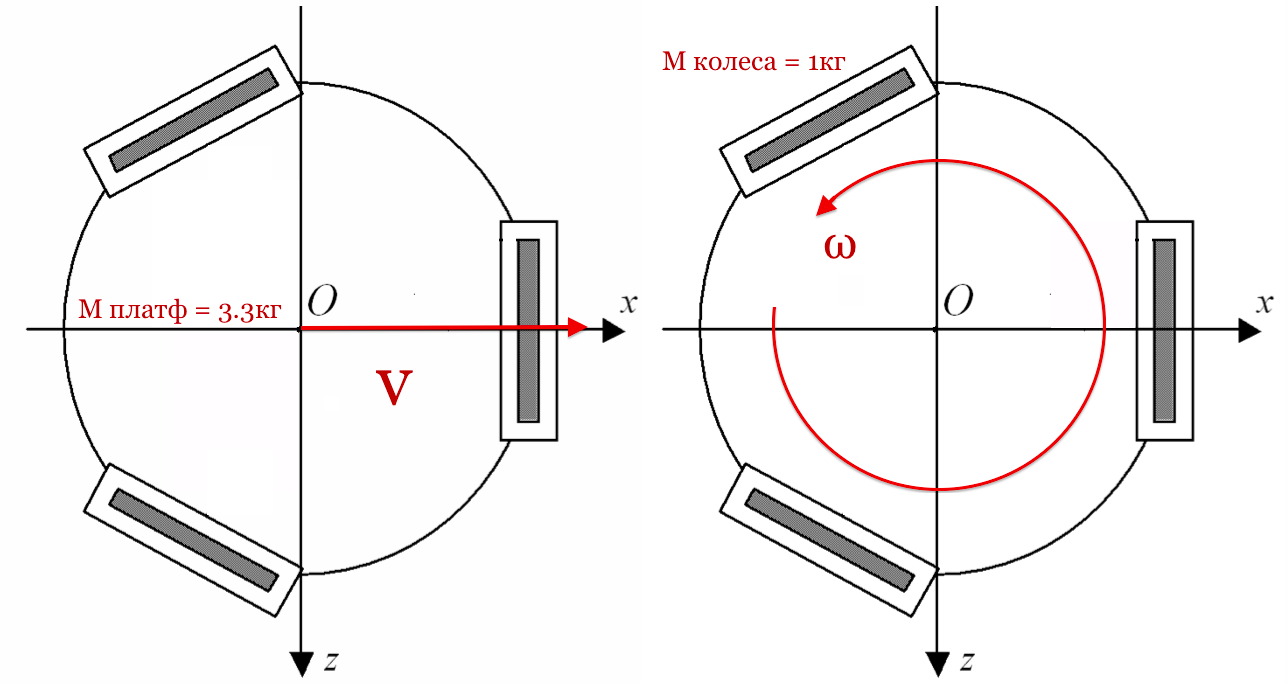
\includegraphics[width=0.95\textwidth]{content/parts/3_friction/diploma/img/art/my_exp_setup.png}
%     \caption{Параметры экспериментов}
%     \label{fig:my_exp_setup}
% \end{figure}

\begin{figure}
    \centering
    \begin{subfigure}[t]{0.3\textwidth}
        \centering
        \asyinclude{content/pic/asy/pic_nu_self_rot.asy}
        \caption{Движение $1$}
        \label{fig:nu_fric_1}
    \end{subfigure}
    \quad
    \begin{subfigure}[t]{0.3\textwidth}
        \centering
        \asyinclude{content/pic/asy/pic_nu_straight.asy}
        \caption{Движение $2$}
        \label{fig:nu_fric_2}
    \end{subfigure}
    \quad
    \begin{subfigure}[t]{0.3\textwidth}
        \centering
        \asyinclude{content/pic/asy/pic_nu_wrench.asy}
        \caption{Движение $3$}
        \label{fig:nu_fric_3}
    \end{subfigure}
    \caption{Рассмотренные варианты начальных условий для моделей с трением. Для модели с сухим трением приведены результаты экспериментов с движениями 1 и 2. Для модели с вязким трением приведены результаты экспериментов с движением 3.}
    \label{fig:nu_fric}
\end{figure}

Для сравнения модели экипажа на плоскости с сухим трением и безынерционной модели с неголономными связями, в таблице\upr{tab:verif} приведены величины отличий угла курса $\theta$ экипажа и координат центра масс $x, y$ к моменту безразмерного времени $t = 10$. Отличия уменьшаются с уменьшением порядка величины отношения массы одного ролика $m_{\text{рол}}$ к суммарной массе колеса $m_{\text{к}}$.

\begin{table}[ht]
    \centering
    \begin{tabular}{l|l|l}
     & Движение $1$ & Движение $2$ \\ \hline
    $\frac{m_{\text{рол}}}{m_{\text{к}}}$ &
    $\Delta \theta$ &
    $\max(|\Delta x|, |\Delta y|)$ \\ \hline
    $10^{-1}$ & $\approx 1$       & $\approx 1$       \\
    $10^{-2}$ & $\approx 10^{-1}$ & $\approx 0.5$     \\
    $10^{-3}$ & $\approx 10^{-2}$ & $\approx 10^{-1}$ \\
    $10^{-4}$ & $\approx 10^{-3}$ & $\approx 10^{-2}$ \\
    $10^{-5}$ & $\approx 10^{-3}$ &                   \\
    $10^{-6}$ & $\approx 10^{-4}$ & 
    \end{tabular}
    \caption{Сравнение моделей экипажа на плоскости с сухим трением и безынерционной модели с неголономными связями. Порядок различий в значениях угла курса платформы $\theta$ и координат центра масс $x, y$ экипажа при движениях $1$ и $2$ и уменьшении $\massrel$}
    \label{tab:verif}
\end{table}

На рис.~\ref{fig:exp_examples} приведены примеры траекторий центра масс $y(x)$ и зависимостей $\theta(t)$ угла поворота $\theta$ платформы вокруг вертикальной оси, проходящей через её центр, для случаев 1) и 2). Кривые $y(x)$, изображающие траектории центра масс, соответствуют, в сущности, точке -- началу системы отсчета $OXYZ$ -- в случае $v_0 = 0, \omega_0 = 1$, и отрезку прямой, совпадающей с осью $x$, в случае $v_0 = 1, \omega_0 = 0$, т.к. масштаб отображения таков, чтобы были видны отклонения от точных значений, возникающие в силу вычислительной погрешности, но сами эти отклонения имеют порядок малости, позволяющий считать их несущественными. Аналогичное утверждение верно и для зависимости угла поворота платформы $\theta$ от времени в случае поступательного движения -- полученная зависимость близка к постоянной.

На рис.~\ref{fig:exp_examples} представлены результаты нескольких численных экспериментов. Во всех случаях величины $x, y$ и $\theta$, демонстрируют поведение, не различимое в масштабе рисунка, и поэтому приведены лишь расхождения между построенной нами моделью и верификационной идеализацией, которые и представляют интерес. Также представлена абсолютная величина скорости скольжения в точке контакта в физической модели.

Графики зависимости скорости скольжения от времени показывают, что скольжение всегда имеет место в окрестности момента смены роликов и только там. Для вращательного движения это объясняется наличием того же динамического эффекта раскручивания роликов, что был обнаружен в главах 1 и 2: скользят именно вновь входящие в контакт ролики, но не ролики, уже находящиеся в контакте достаточное время. В случае поступательного движения платформы экипажа дополнительно возникает раскручивание роликов задних колес, находящихся в контакте, поскольку для идеального качения при подходе к острию, ролику необходима бесконечная угловая скорость собственного вращения, т.к. его радиус вблизи острия стремится к нулю.

Из рис.~\ref{fig:exp_examples_1_12}--\ref{fig:exp_examples_2_34} видно, что с ростом доли массы роликов в общей массе колеса скольжение в контакте становится существеннее, изменяясь от пренебрежимо малого при $\massrel = 10^{-6}$ до весьма заметного уже при $\massrel = 10^{-3}$. Тем не менее, расхождения в сравниваемых моделях траектории центра масс и угла поворота платформы малы. Скольжение наблюдается лишь в точках колеса, которые в промышленных конструкциях не присутствуют (см. Обзор), что и позволяет считать построенную модель экипажа на плоскости с сухим трением верифицированной.

% В процессе отладки модели рассматривались автономные движения отдельного омни-колеса.

На рис.~\ref{fig1} представлены зависимости расстояний $h$ между горизонтальной плоскостью и роликами одного и того же колеса, находящимися в разных фазах (перед контактом, в контакте, после контакта). Номер кривой соответствует номеру ролика на колесе. В увеличенном масштабе показан момент смены ролика в контакте с опорной плоскостью. Видно, что характер смены гладкий безударный.

\begin{figure}[htb]
    \centerline{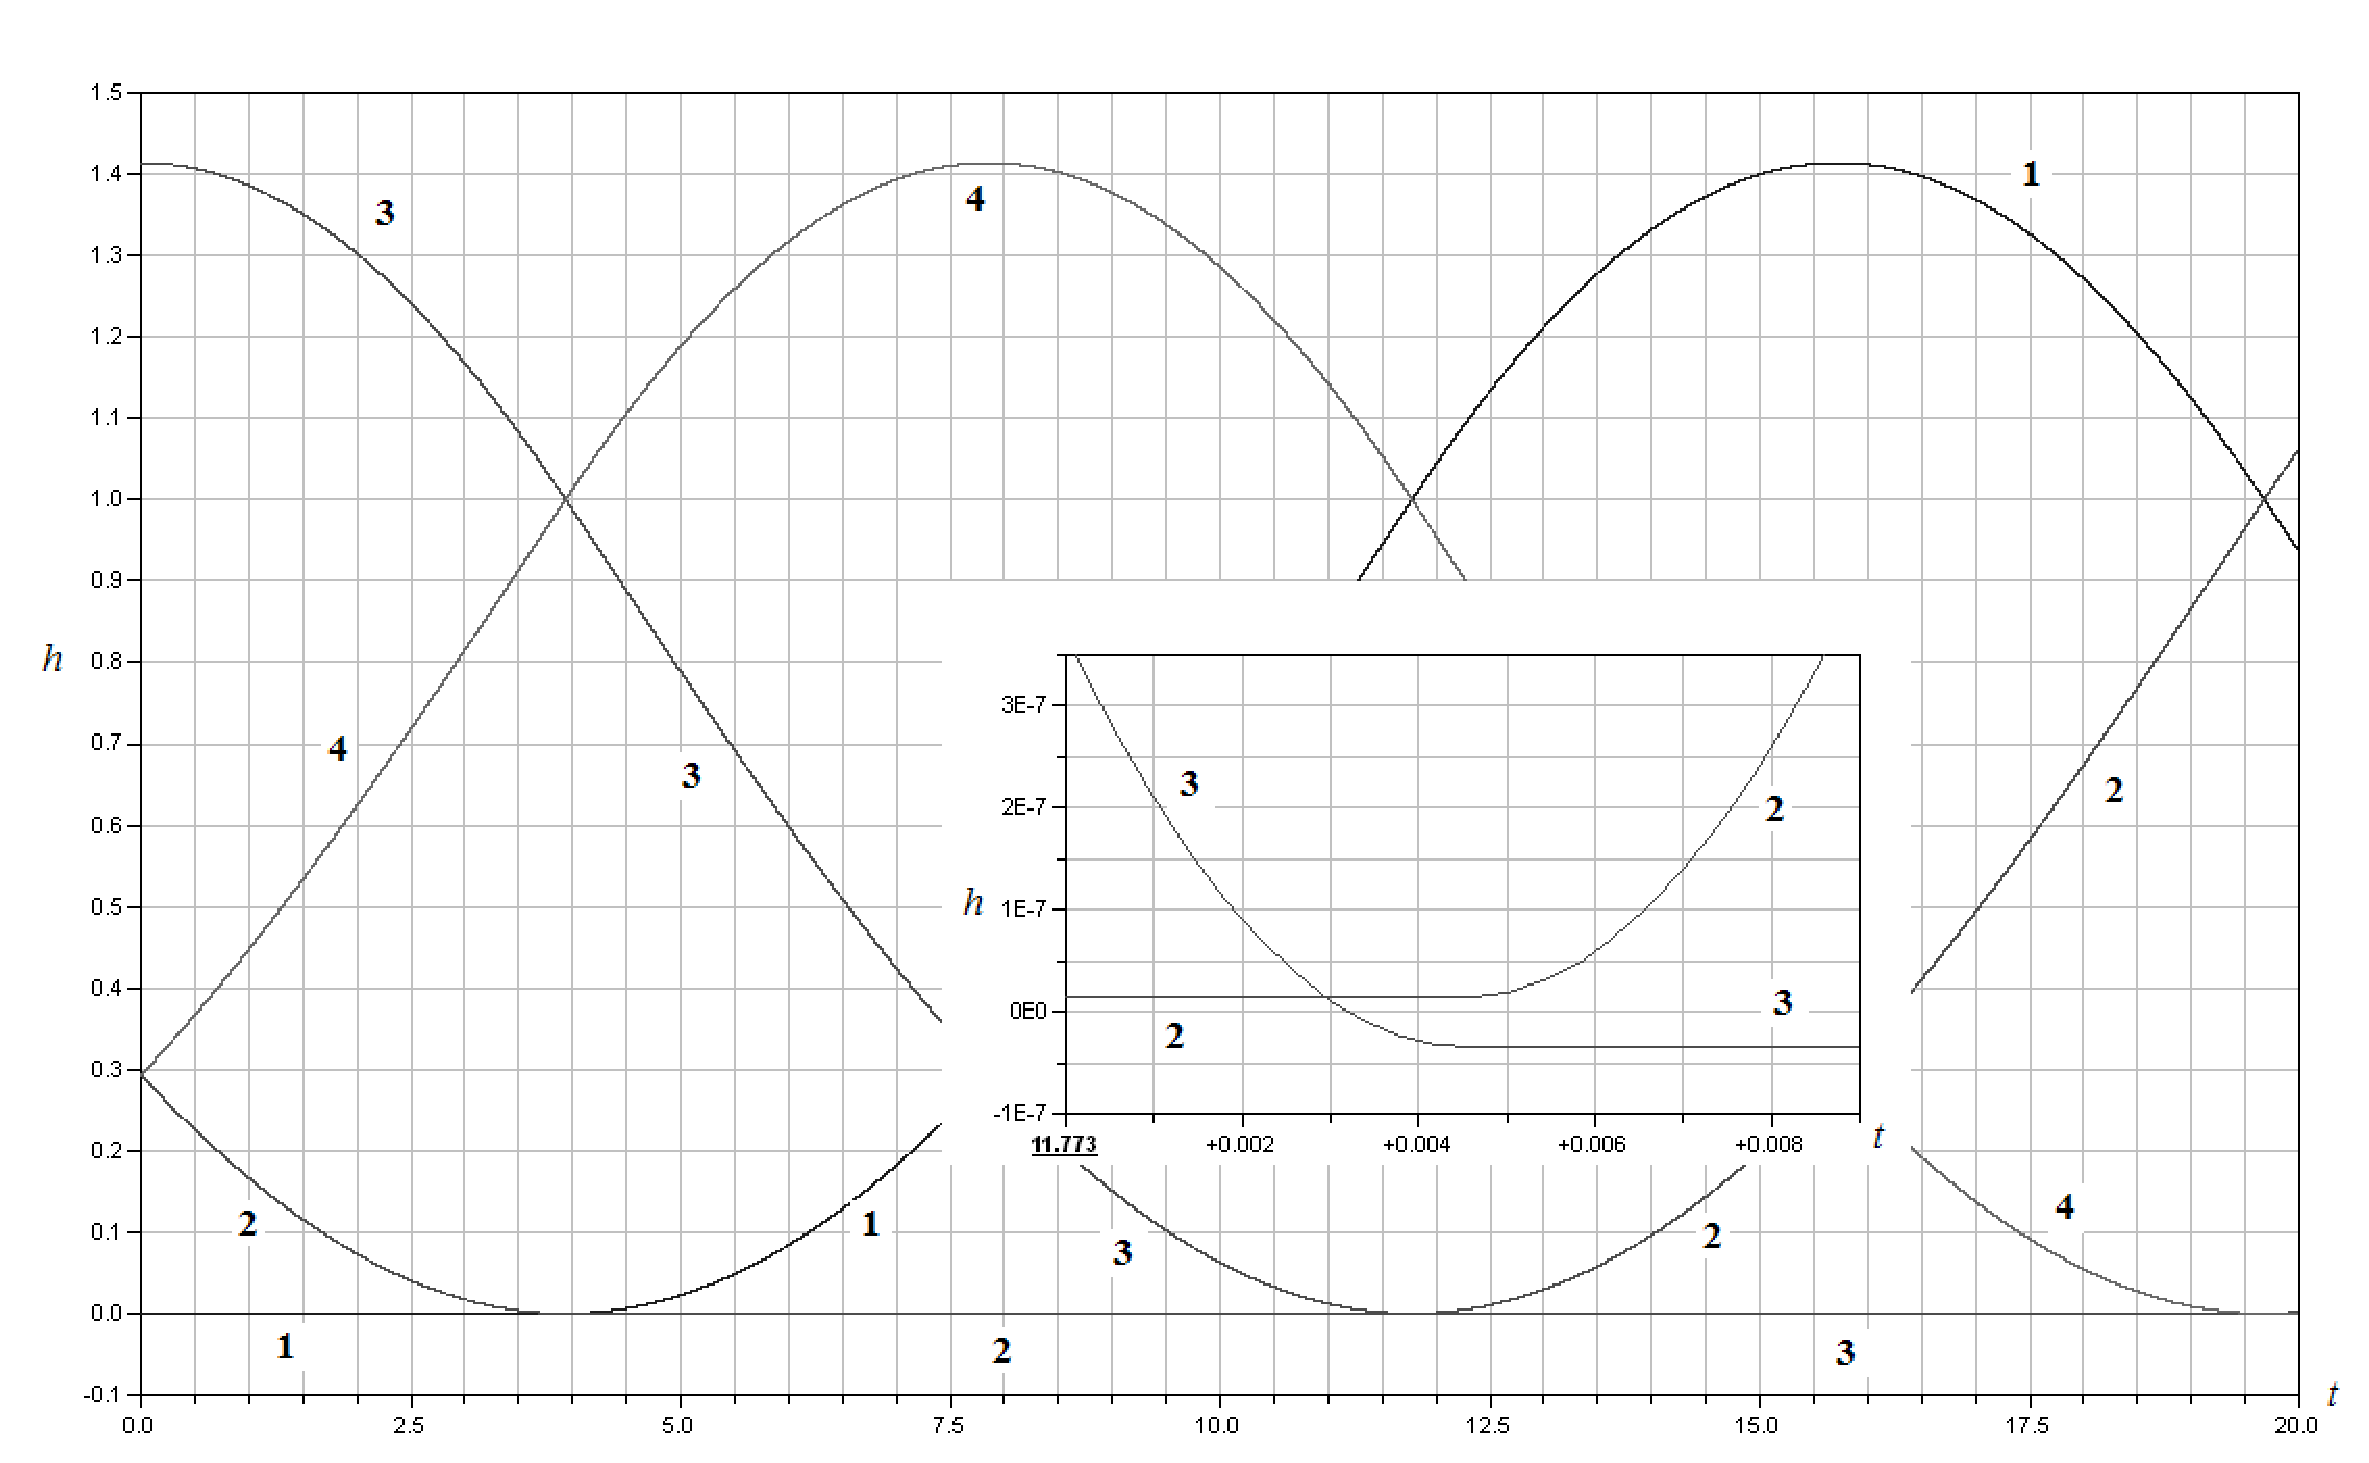
\includegraphics[width=15cm]{content/parts/3_friction/nd/Figure11.eps}}
    \caption{Процесс смены роликов в контакте в численной модели.}
    \label{fig1}
\end{figure}

Одновременно можно наблюдать, что неудерживающая связь \\ (рис.~\ref{fig:precis}), реализуется достаточно точно, несмотря на постепенное увеличение вычислительной ошибки. Расстояние между контактирующими телами медленно увеличивается для каждого последующего ролика в контакте. В то же время, абсолютная величина ошибки остается пренебрежимо малой -- около $10^{-7}$ от единицы безразмерной длины. 

\begin{figure}[htb]
    \centerline{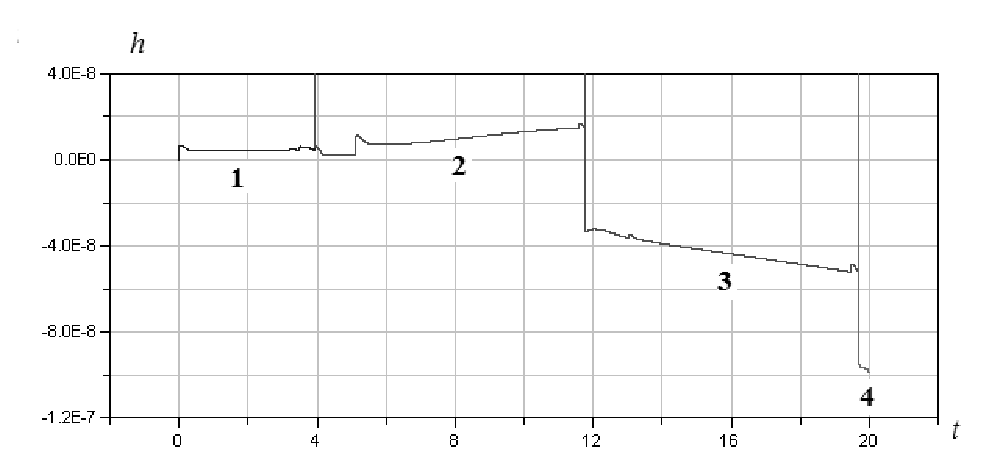
\includegraphics[width=15cm]{content/parts/3_friction/nd/Figure21.eps}}
    \caption{Точность сохранения неудерживающей связи.}
    \label{fig:precis}
\end{figure}

\subsection{Качественное сравнение модели с вязким трением и безынерционной модели}

Для модели с вязким трением были проведены расчеты, аналогичные движению 3 из главы 2. Конфигурация экипажа также симметрична, ролики усечены, на каждом колесе пять роликов.

Обнаружены динамические эффекты, аналогичные полученным в главе 2: характерный спиральный вид траектории центра масс на опорной плоскости возникает и в данной модели; видно раскручивание роликов; возрастание угловой скорости платформы экипажа, одновременное с убыванием поступательной скорости её центра; последующее медленное убывание угловой скорости; убывание кинетической энергии экипажа, см. рис.~\ref{fig:viscous}.

В данном расчете коэффициент вязкого трения принимался достаточно большим: $10^{5}$. Такое значение позволило моделировать ударный характер переходных процессов при смене ролика в контакте. На гладких участках движения сходство с движением неголономной модели соответствует результату \cite{karapetyan1981negolonom}.

Подведем итог описанным в настоящей главе исследованиям: построена модель экипажа с неидеальными голономными связями. Модель реализована в системе автоматического построения численных динамических моделей для двух моделей контактных сил: вязкого трения и регуляризованного сухого трения. Для этого найдены геометрические условия контакта роликов омни- и mecanum-колес и опорной плоскости. Численно показано, что при стремлении осевого момента инерции ролика к нулю, движения системы с трением стремятся к движениям безынерционной модели. Обнаружено качественное сходство траекторий системы с вязким трением с достаточно большим коэффициентом трения с движениями модели, рассмотренной в главах 1 и 2.

% \vspace{50pt}

% \newpage

% EXAMPLES
\begin{figure}[ht]
    \centering
    \begin{subfigure}{.47\textwidth}
        \centering
        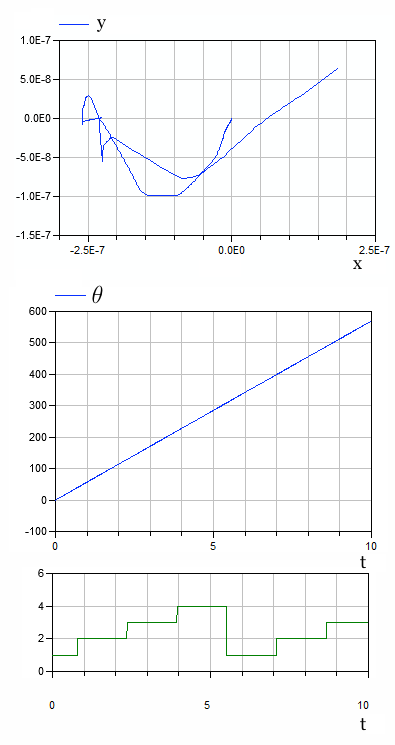
\includegraphics[width=\textwidth]{content/pic/new/dry/example_v_0_0_omega_1_frac_1e-1_n_4_time_10s.png}
        \caption{$\massrel = 0,1, v_0 = 0, \omega_0 = 1$}
        \label{fig:exp_example_omega}
    \end{subfigure}%
    \hspace{5pt}
    \begin{subfigure}{.47\textwidth}
        \centering
        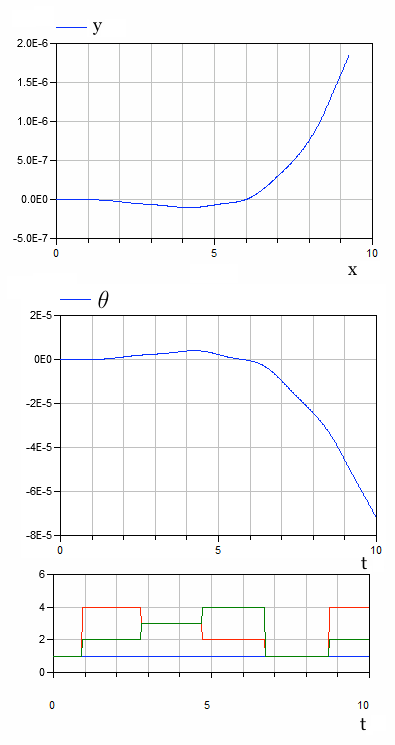
\includegraphics[width=\textwidth]{content/pic/new/dry/example_v_1_0_omega_0_frac_1e-1_n_4_time_10s.png}
        \caption{$\massrel = 0,1, v_0 = 1, \omega_0 = 0$}
        \label{fig:exp_example_v}
    \end{subfigure}
    \caption{Примеры траекторий центра масс экипажа, зависимости угла курса $\theta$ от времени и смены номеров роликов в контакте для двух типов начальных условий. На нижнем графике - номер ролика в контакте, см. также рис.~\ref{fig:wheel}}
    \label{fig:exp_examples}
\end{figure}
\newpage

\begin{figure}[ht]
    \begin{center}\begin{equation*}\begin{array}{cc}
    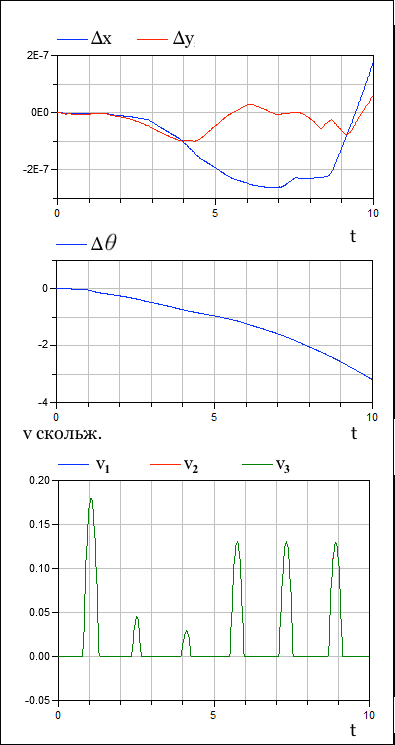
\includegraphics[width=7cm, viewport=0 0 395 745,clip]{content/pic/new/dry/comparison_v_0_0_omega_1_frac_1e-1_n_4_time_10s.png} & 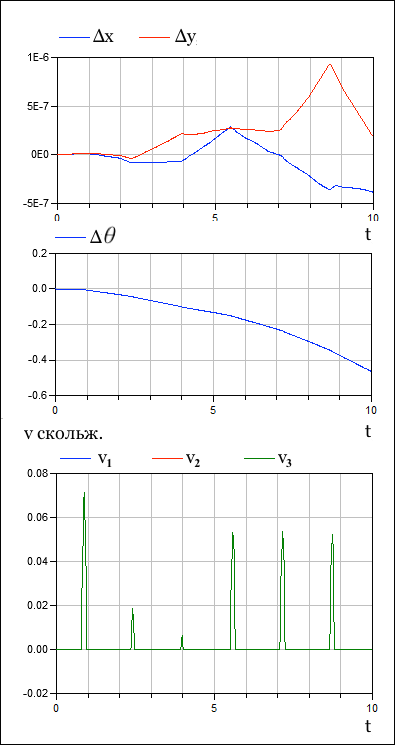
\includegraphics[width=7cm, viewport=0 0 395 745,clip]{content/pic/new/dry/comparison_v_0_0_omega_1_frac_1e-2_n_4_time_10s.png}\\
    \massrel = 10^{-1}, v_0 = 0, \omega_0 = 1 & \massrel = 10^{-2}, v_0 = 0, \omega_0 = 1\\
    \end{array}\end{equation*}\end{center}
    \caption{Движение 1 экипажа на плоскости с сухим трением, $\massrel = 10^{-1}, 10^{-2}$. Траектории центра масс $y(x)$, зависимости $\theta(t)$ угла курса от времени и абсолютны величины скоростей скольжения в точках контакта.}
    \label{fig:exp_examples_1_12}
\end{figure}
\newpage

\begin{figure}[ht]
    \begin{center}\begin{equation*}\begin{array}{cc}
    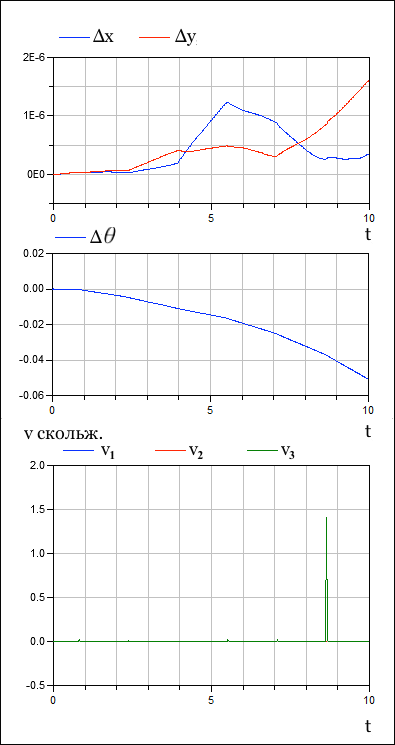
\includegraphics[width=7cm, viewport=0 0 395 745,clip]{content/pic/new/dry/comparison_v_0_0_omega_1_frac_1e-3_n_4_time_10s.png} & 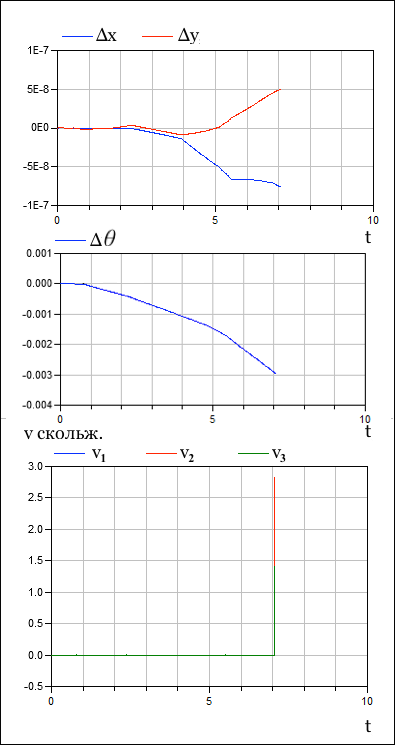
\includegraphics[width=7cm, viewport=0 0 395 745,clip]{content/pic/new/dry/comparison_v_0_0_omega_1_frac_1e-4_n_4_time_10s.png}\\
    \massrel = 10^{-3}, v_0 = 0, \omega_0 = 1 & \massrel = 10^{-4}, v_0 = 0, \omega_0 = 1\\
    \end{array}\end{equation*}\end{center}
    \caption{Движение 1 экипажа на плоскости с сухим трением, $\massrel = 10^{-3}, 10^{-4}$. Типы графиков те же, что на рис.~\ref{fig:exp_examples_1_12}.}
    \label{fig:exp_examples_1_34}
\end{figure}
\newpage

\begin{figure}[ht]
    \begin{center}\begin{equation*}\begin{array}{cc}
    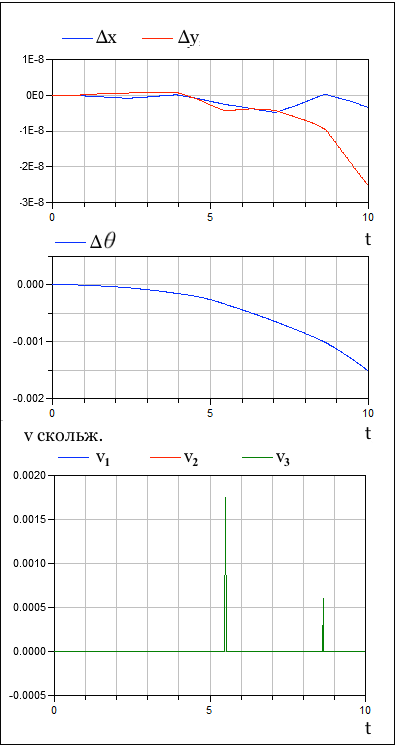
\includegraphics[width=7cm, viewport=0 0 395 745,clip]{content/pic/new/dry/comparison_v_0_0_omega_1_frac_1e-5_n_4_time_10s.png} & 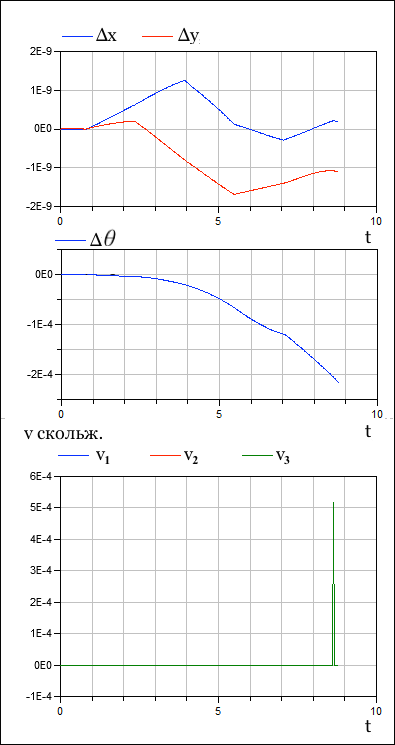
\includegraphics[width=7cm, viewport=0 0 395 745,clip]{content/pic/new/dry/comparison_v_0_0_omega_1_frac_1e-6_n_4_time_10s.png}\\
    \massrel = 10^{-5}, v_0 = 0, \omega_0 = 1 & \massrel = 10^{-6}, v_0 = 0, \omega_0 = 1\\
    \end{array}\end{equation*}\end{center}
    \caption{Движение 1 экипажа на плоскости с сухим трением, $\massrel = 10^{-5}, 10^{-6}$. Типы графиков те же, что на рис.~\ref{fig:exp_examples_1_12}.}
    \label{fig:exp_examples_1_56}
\end{figure}
\newpage

\begin{figure}[ht]
    \begin{center}\begin{equation*}\begin{array}{cc}
    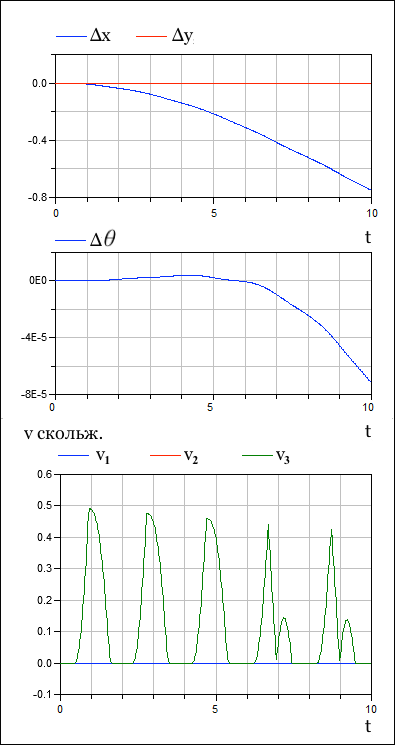
\includegraphics[width=7cm, viewport=0 0 395 745,clip]{content/pic/new/dry/comparison_v_1_0_omega_0_frac_1e-1_n_4_time_10s.png} & 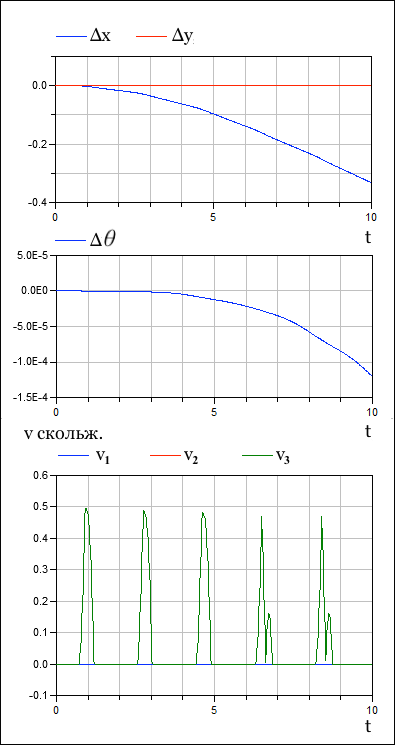
\includegraphics[width=7cm, viewport=0 0 395 745,clip]{content/pic/new/dry/comparison_v_1_0_omega_0_frac_1e-2_n_4_time_10s.png}\\
    \massrel = 10^{-1}, v_0 = 1, \omega_0 = 0 & \massrel = 10^{-2}, v_0 = 1, \omega_0 = 0\\
    \end{array}\end{equation*}\end{center}
    \caption{Движение 2 экипажа на плоскости с сухим трением, $\massrel = 10^{-1}, 10^{-2}$. Типы графиков те же, что на рис.~\ref{fig:exp_examples_1_12}.}
    \label{fig:exp_examples_2_12}
\end{figure}
\newpage

\begin{figure}[htb]
\begin{center}\begin{equation*}\begin{array}{cc}
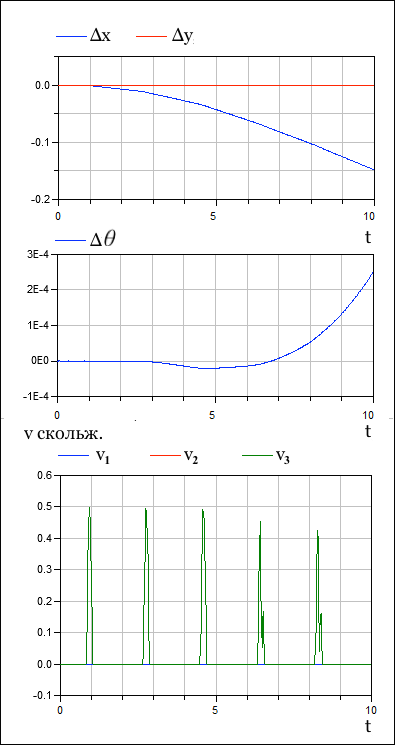
\includegraphics[width=7cm, viewport=0 0 395 745,clip]{content/pic/new/dry/comparison_v_1_0_omega_0_frac_1e-3_n_4_time_10s.png} & 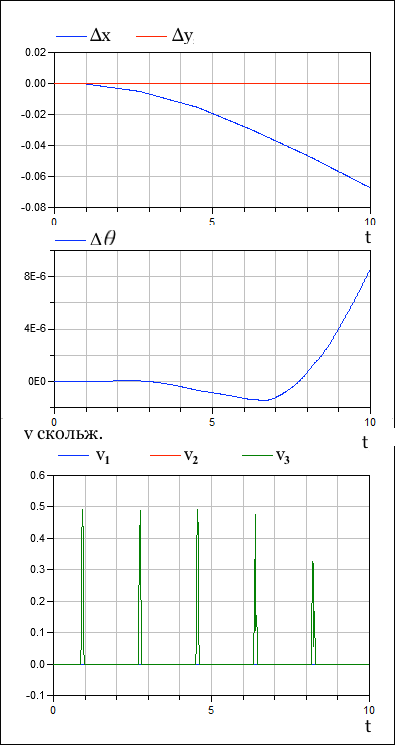
\includegraphics[width=7cm, viewport=0 0 395 745,clip]{content/pic/new/dry/comparison_v_1_0_omega_0_frac_1e-4_n_4_time_10s.png}\\
\massrel = 10^{-3}, v_0 = 1, \omega_0 = 0 & \massrel = 10^{-4}, v_0 = 1, \omega_0 = 0\\
\end{array}\end{equation*}\end{center}
\caption{Движение 1 экипажа на плоскости с сухим трением, $\massrel = 10^{-3}, 10^{-4}$. Типы графиков те же, что на рис.~\ref{fig:exp_examples_1_12}.}
\label{fig:exp_examples_2_34}
\end{figure}
\newpage

\begin{figure}[htb]
    \centering
    \minipage{0.45\textwidth}
        \begin{subfigure}[t]{\textwidth}
            \centering
            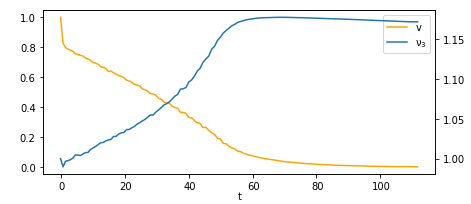
\includegraphics[width=\linewidth]{content/pic/new/viscous/visc_3_100_vnu3.png}
            \vspace{-25pt}
            \caption{Абсолютная величина $v$ скорости центра масс экипажа и угловая скорость платформы $\nu_3$}
            \label{fig:visc_vnu3}
        \end{subfigure}
        \begin{subfigure}[t]{\textwidth}
            \vspace{15pt}
            \centering
            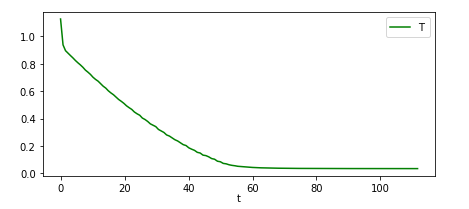
\includegraphics[width=\linewidth]{content/pic/new/viscous/visc_3_100_T.png}
            \vspace{-25pt}
            \caption{Кинетическая энергия экипажа}
            \label{fig:visc_T}
        \end{subfigure}
        \begin{subfigure}[t]{\textwidth}
            \vspace{15pt}
            \centering
            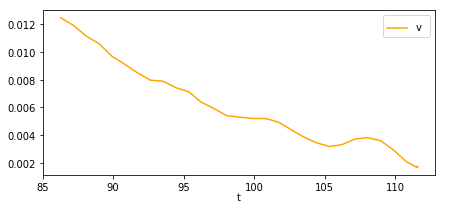
\includegraphics[width=\linewidth]{content/pic/new/viscous/visc_3_100_v_late.png}
            \vspace{-25pt}
            \caption{Абсолютная величина $v$ скорости центра масс экипажа на интервале $t > 85$}
            \label{fig:visc_v_late}
        \end{subfigure}
    \endminipage
    \quad
    \minipage{0.45\textwidth}
        \begin{subfigure}[t]{\textwidth}
            \centering
            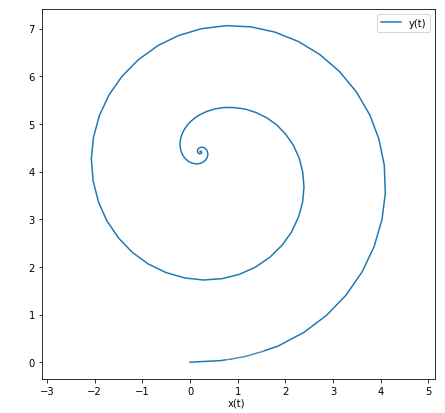
\includegraphics[width=\linewidth]{content/pic/new/viscous/visc_3_100_traj.png}
            \vspace{-25pt}
            \caption{Траектория центра масс экипажа на плоскости $OXY$}
            \label{fig:visc_traj}
        \end{subfigure}
        \begin{subfigure}[t]{\textwidth}
            \vspace{20pt}
            \centering
            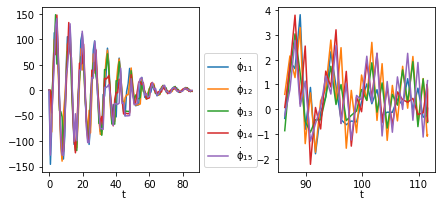
\includegraphics[width=\linewidth]{content/pic/new/viscous/visc_3_100_dphi.png}
            \vspace{-25pt}
            \caption{Угловые скорости роликов на колесе номер 1. Слева -- на интервале $t < 85$, справа -- на следующем интервале.}
            \label{fig:visc_dphi}
        \end{subfigure}
    \endminipage

    \caption{Характер движения системы с вязким трением при комбинации начальных условий движений 1 и 2. По оси абсцисс всюду, кроме графика \ref{fig:visc_traj}, отложено безразмерное время $t$.}
    \label{fig:viscous}
\end{figure}
